\section{Fichiers exécutables et Processus}
\subsection{Fichier binaire et fichier texte}
\begin{frame}{Fichier binaire et fichier texte}
  \begin{columns}
    \begin{column}{5cm}
      \begin{block}{Les données numériques}
        Tout fichier enregistré sur un support numérique est une suite
        d'octets.
      \end{block}
    \end{column}
    \begin{column}{6cm}
      \begin{center}
        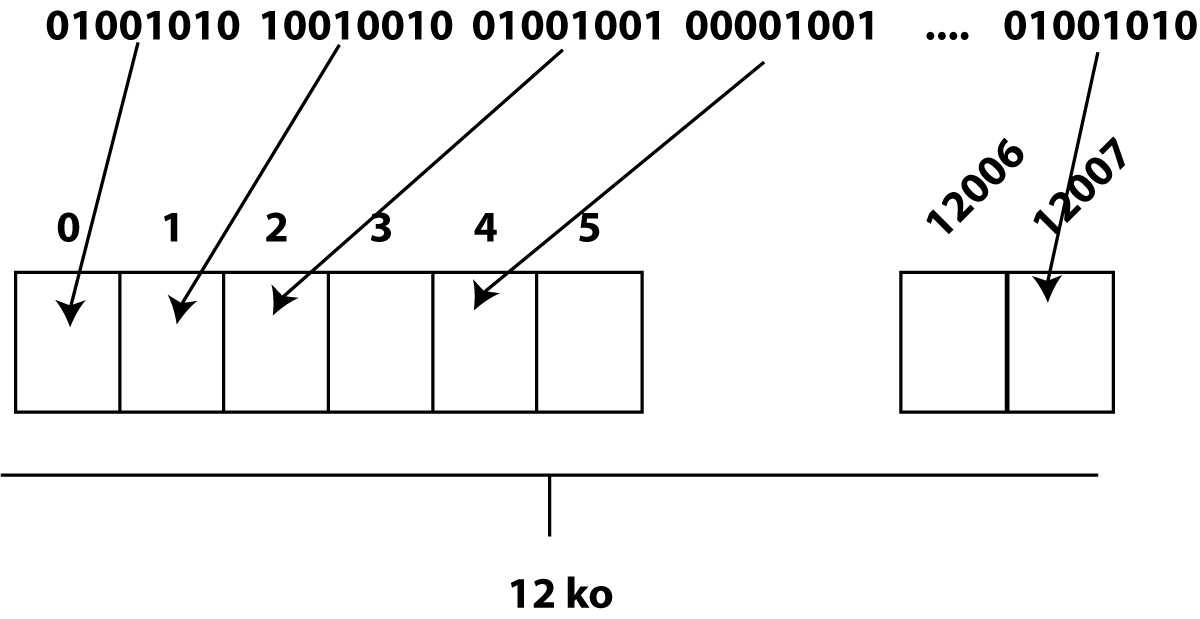
\includegraphics[width=4cm]{img/s03/Memoire.jpg}
      \end{center}
    \end{column}
  \end{columns}
  \begin{center}
    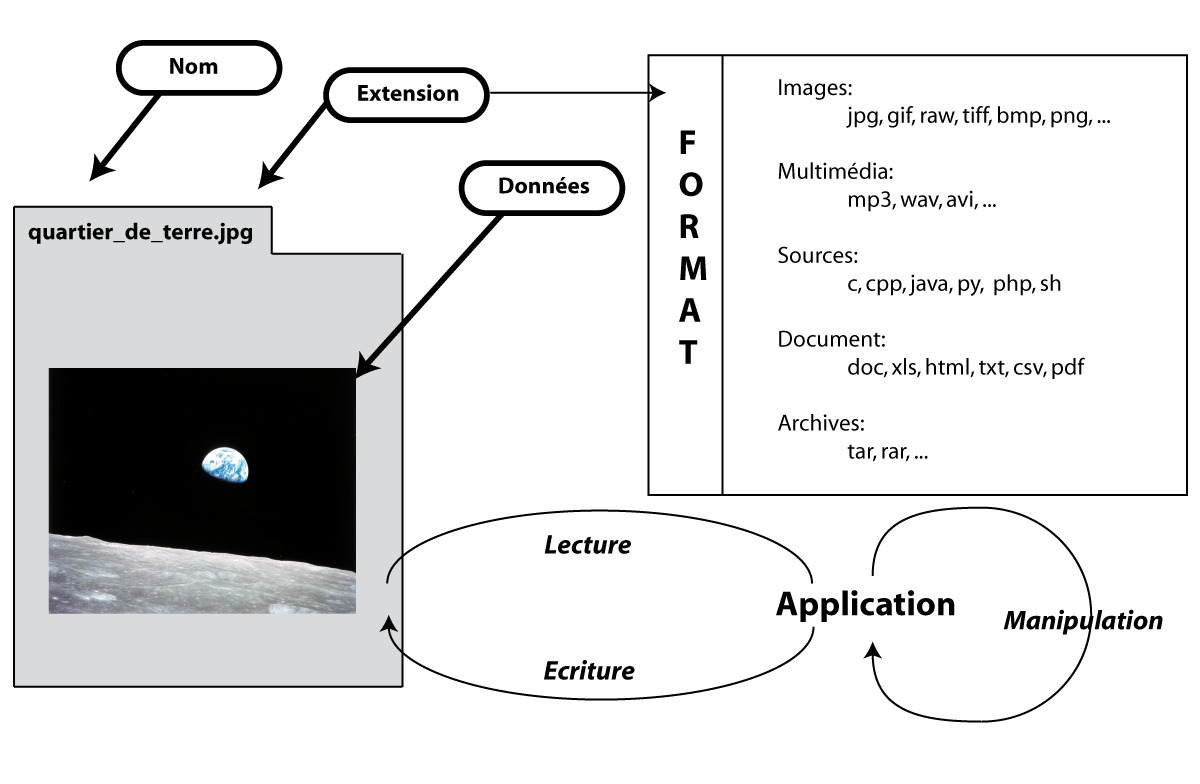
\includegraphics[height=4cm]{img/s03/fichier_1_1.jpg}
    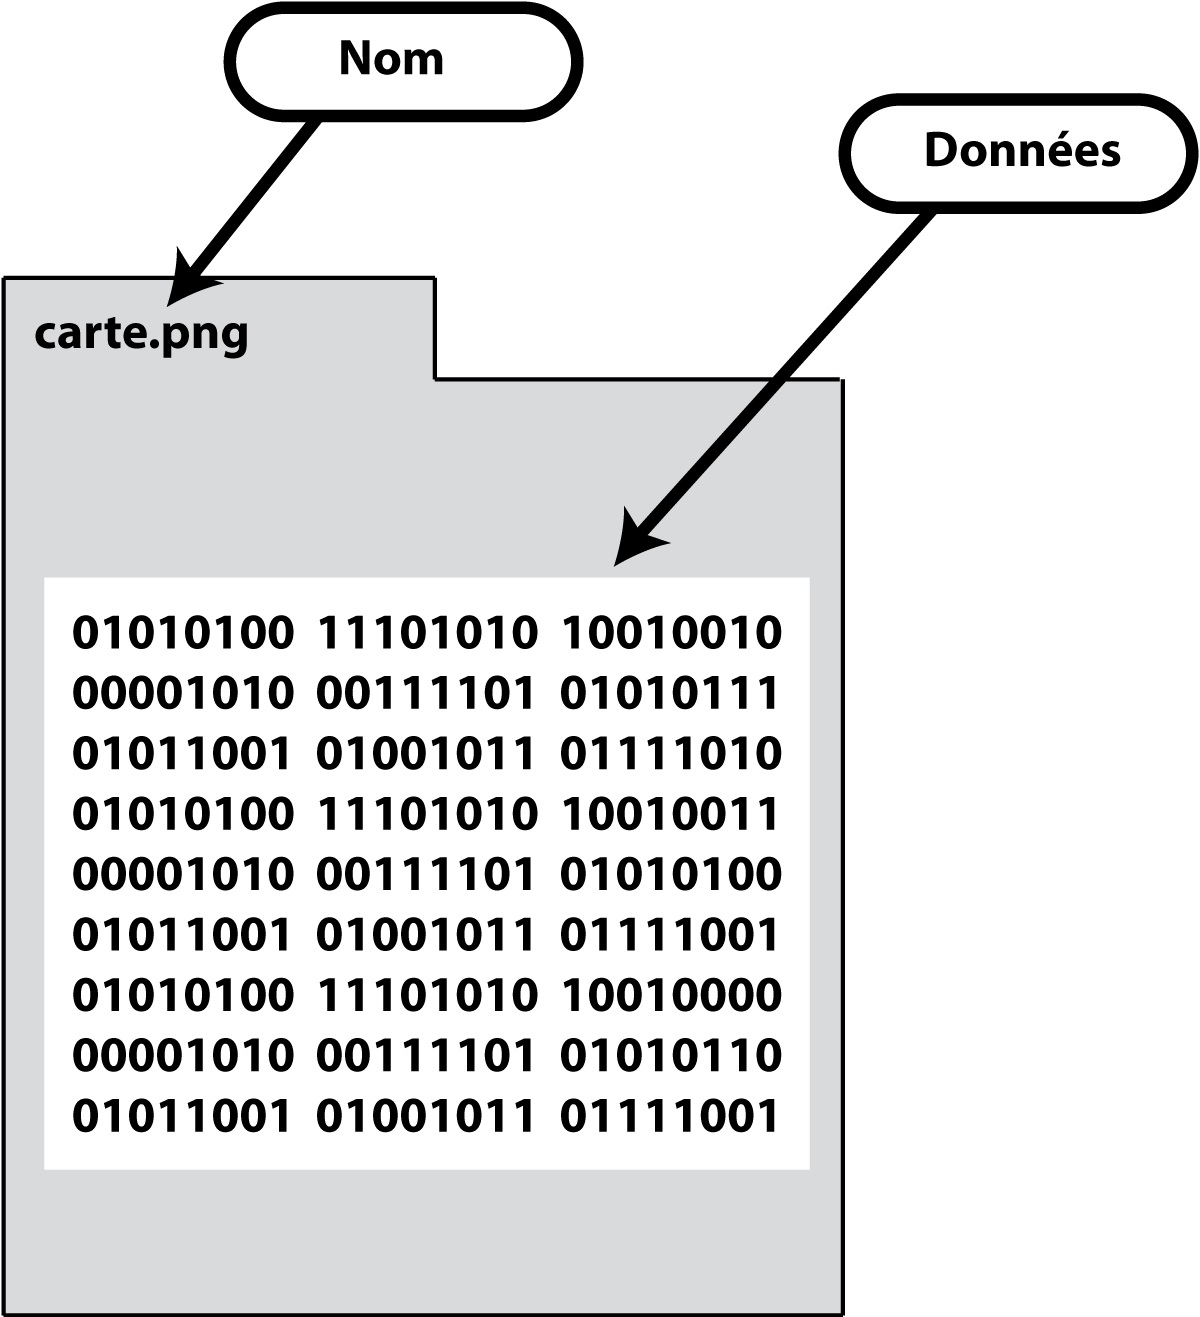
\includegraphics[height=3cm]{img/s03/fichier_1.jpg}
  \end{center}
  \begin{block}{Accès aux données}
    Lors de son utilisation un fichier est \textit{lu} par un
    programme. Pour cela il doit décoder les informations binaires et
    les traiter.
  \end{block}
\end{frame}

\begin{frame}{Fichier binaire et fichier texte}
  \begin{block}{Deux grands types de fichiers: Binaire Vs Numérique}
    De façon générale un fichier binaire ne peut être \textit{"lu"} que
    par un programme informatique, alors qu'un fichier texte peut être
    \textit{"lu"} par être humain.
  \end{block}
  \begin{columns}
    \begin{column}{6cm}
      \begin{block}{Les fichiers textes}
        C'est un fichier qui peut être \textit{"lu"} par un éditeur de
        texte brut. Les données sont encodées comme une suite de
        caractères.
      \end{block}
      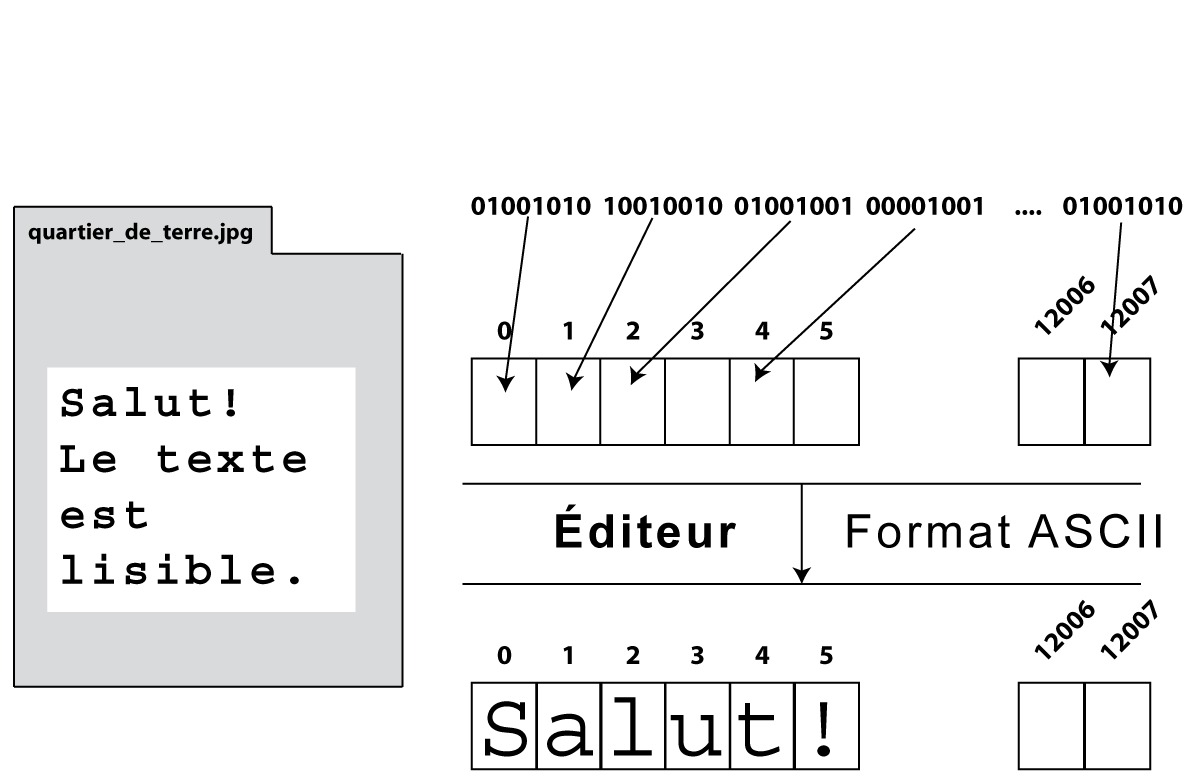
\includegraphics[width=6cm]{img/s03/fichier_1_3.jpg}
    \end{column}
    \begin{column}{6cm}
      \begin{block}{Les fichiers binaires}
        Ce n'est pas un fichier texte \dots Il peut contenir des
        instructions machines, des données compressées, des données
        binaires brutes nécessitant un programme pour être lues.
      \end{block}
      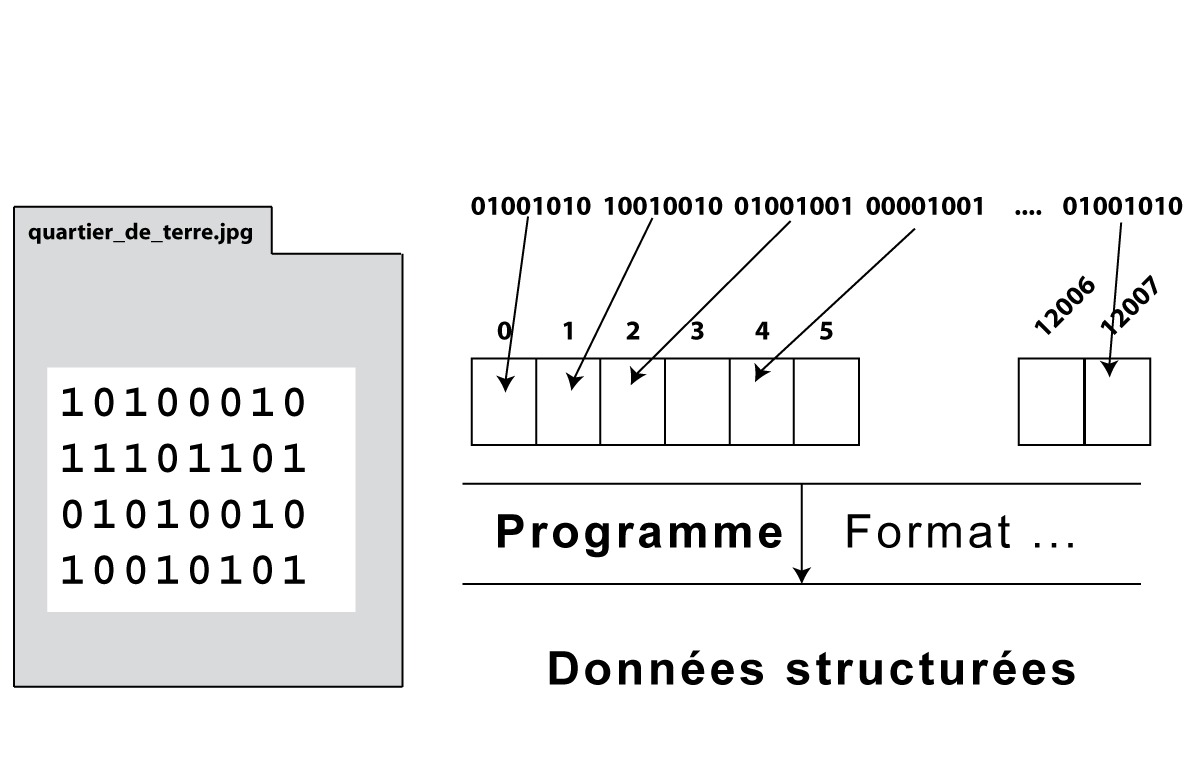
\includegraphics[width=6cm]{img/s03/fichier_1_4.jpg}
    \end{column}
  \end{columns}
\end{frame}
\begin{frame}{Fichiers sources \textrightarrow Exécutable
    \textrightarrow Processus}

  \begin{columns}
    \begin{column}{3.8cm}
      \begin{block}{Les sources: Une \textit{"recette de cuisine"}}
        \begin{itemize}
        \item Exprime un ensemble de tâches à réaliser pour accomplir le
          programme (le plat cuisiné).
        \item Utilise un langage de programmation.
        \item C'est un fichier texte.
        \end{itemize}
      \end{block}
      \fileform[3cm]{dessine.c}{%
        (\dots)\\
        float r, x, y;\\
        r=3.0;\\
        x=0.0;\\
        y=7.1;\\
        cercle(0,0,,r)\\
        segment(0,0,x,y)}
    \end{column}
    \begin{column}{3.8cm}
      \begin{block}{L'exécutable}
        \begin{itemize}
        \item Exprime les mêmes tâches dans un langage machine.
        \item Ce fichier ne fonctionne que sur des ordinateurs qui ont
          la même architecture.
        \item C'est un fichier binaire.
        \end{itemize}
      \end{block}
      \vfill \fileform[3cm]{dessine}{%
        10100101 11101001\\
        10001001 00100101\\
        00101010 00100010\\
        01111011 10110101\\
        01000010 00110011\\
        00101101 11010100\\
        (\dots)}
    \end{column}
    \begin{column}{3.8cm}
      \begin{block}{Les processus}
        \begin{itemize}
        \item L'évaluation des instructions machines engendre des
          processus.
        \item Ces processus sont exécutés par le matériel.
        \item Les instructions machine doivent donc être adaptées au
          matériel.
        \end{itemize}
      \end{block}
      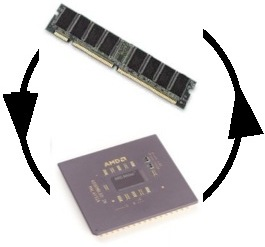
\includegraphics[width=3.5cm]{img/s03/fichier_1_5.jpg}
    \end{column}
  \end{columns}
\end{frame}
\begin{exercice}
  \begin{exercicelet}{Préparation}
    \begin{enumerate}\setcounter{enumi}{\value{cnti}}
    \item Vérifiez que votre répertoire courant est bien
      \verb|TP_2|. Analysez l'affichage produit par la commande ls
      suivie des options \texttt{-lh}. Vous pourrez comparer les
      affichages obtenus par les commandes \texttt{ls -l} et \texttt{ls
        -lh} pour comprendre l'effet de l'option \texttt{-h}. Vous
      pourrez aussi rechercher cette information dans les pages de man.
    \item Analysez l'arborescence créée lors de l'extraction des données
      de l'archive au moyen de la commande \texttt{ls}. Vous dessinerez
      cette arborescence.
    \item Après vous être placé dans le répertoire créé lors de
      l'extraction de l'archive (donnees), quelle commande permet
      d'identifier le plus gros fichier (taille mémoire). Identifiez-le.
    \item Quelles commandes vous permettent d'afficher le contenu des
      fichiers texte \verb|command_line.txt| et \texttt{0readme}? Quels
      sont leurs contenus?
    \item Analysez le résulat de l'évaluation des commandes suivantes:
\begin{verbatim}
 file 0readme
 file commande_line.txt
 file images/solar.png
\end{verbatim}
    \item Quelle est la fonction de la commande \texttt{file}? Parcourez
      les pages de manuel de cette commande.
      \setcounter{cnti}{\value{enumi}}
    \end{enumerate}
  \end{exercicelet}
\end{exercice}

\subsection{Processus dans un système multitâches et mutli-utilisateurs}
\begin{frame}{Identification des processus par le système
    d'exploitation}
  \begin{block}{Système multi-utilisateur}
    \begin{itemize}
    \item Plusieurs utilisateurs partagent les mêmes ressources matériel
      (RAM, CPU, disques, \dots),
    \item Chaque utilisateur lance des processus liés à ses activités
      sur la machine et il utilise les résultats de ces processus.
    \end{itemize}
  \end{block}
  \begin{block}{Système multi-tâches}
    \begin{itemize}
    \item Plusieurs programmes en cours d'exécution partagent les mêmes
      ressources matériel (mémoire vive, CPU, disques, \dots). Ils
      peuvent provenir d'un seul ou de plusieurs utilisateurs,
    \item Chaque programmes lance des processus et il utilise les
      résultats de ces processus.
    \end{itemize}
  \end{block}
  \begin{alertblock}{Il faut partager les ressources !!!}
    \begin{itemize}
    \item Chaque programme doit être exécuté éventuellement \textit{"en
        même temps"}. Il faut donc gérer le partage des ressources de
      calcul (accès à la mémoire vive, au CPU),
    \item Chaque programme ou utilisateur doit pouvoir retrouver les
      résultats de ses calculs. Il faut donc pouvoir identifier qui a
      lancé les processus et qui doit récupérer les résultats.
    \end{itemize}
    La gestion des processus est réalisée par le système
    d'exploitation. C'est une de ses tâches principales. Pour cela il a
    besoin de pouvoir identifier chaque processus.
  \end{alertblock}
\end{frame}
\begin{frame}{PID et PPID}
  \begin{block}{PID - \textbf{P}rocess \textbf{ID}entifier}
    \begin{itemize}
    \item C'est un numéro unique attribué à chaque processus lors de son
      lancement.
    \item Il permet d'identifier de façon unique chaque processus.
    \item La liste des processus en cours d'exécution est accessible en
      ligne de commande par les commandes \lin{ps} et \lin{top}.
    \end{itemize}
  \end{block}
  \begin{block}{PPID - \textbf{P}arent \textbf{P}rocess
      \textbf{ID}entifier}
    \begin{itemize}
    \item Le premier processus lancé porte le numéro de PID 1. Les
      processus suivants sont des processus issus de ce processus
      parent.
    \item Chaque processus est lancé par un processus parent
      \textit{via} l'appel système \lin{fork}.
    \item Le PPID est le PID du processus Parent.
    \end{itemize}
  \end{block}
  \begin{block}{Utilités}
    \begin{itemize}
    \item L'utilisateur peut suivre un processus, le suspendre
      temporairement, le relancer ou le tuer (interruption définitive).
    \item Le système s'en sert pour lui affecter des ressources
      matériel.
    \end{itemize}
  \end{block}
\end{frame}

\begin{exercice}
  \begin{exercicelet}{Racourcis clavier et astuces en ligne de commande}
    \begin{enumerate}\setcounter{enumi}{\value{cnti}}
      \setcounter{cnti}{\value{enumi}}
    \item Tapez les 2 caractères \texttt{sl} puis pressez la touche \Tab
      (Tab). Que se passe-t-il?
    \item Tapez les 3 caractères \texttt{sle} puis pressez la touche
      \Tab. Que se passe-t-il?
    \item À la suite de l'affichage précédent tapez la combinaison de
      touches \Ctrl\keystroke{A}. Que se passe-t-il?
    \item Que fait la commande \texttt{man sleep}? Que pouvez-vous dire
      de la commande \texttt{sleep}?
    \item Exécutez la commande \texttt{sleep 32000000}. Que se
      passe-t-il si vous tapez la combinaison de touches
      \Ctrl\keystroke{C}?
    \item Quelle action produit la pression de la flèche \UArrow sur
      votre clavier?
    \item Quelle est l'action produite par la pression de la combinaison
      de touches \Ctrl\keystroke{U} après avoir tapé quelques lettres?
      Par la combinaison de touche \Ctrl\keystroke{L}?
    \item Quelle est l'action produite en tapant ls\Spacebar\Tab (le
      caractère \Spacebar signifie la présence d'un espace)?
    \end{enumerate}
  \end{exercicelet}
\end{exercice}

\subsection{Gestion de la mémoire vive}
\begin{frame}{Gestion de la mémoire vive}
  \begin{columns}
    \begin{column}{6cm}
      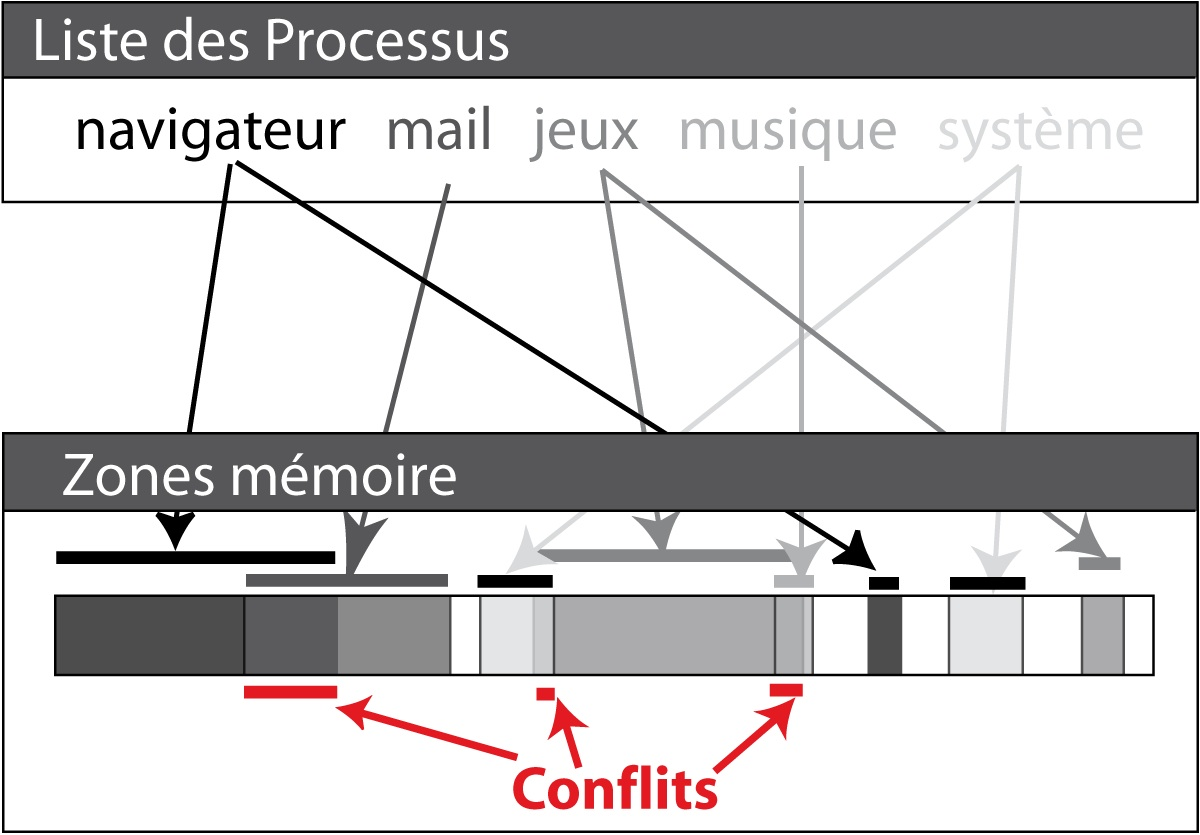
\includegraphics[width=5.5cm]{img/s03/Alloc_mem_1.jpg}
      \begin{block}{Chaque processus a besoin de mémoire}
        Pour stocker et travailler sur:
        \begin{itemize}
        \item les données,
        \item les instructions,
        \item les résultats.
        \end{itemize}
      \end{block}
      \begin{alertblock}{Il faut assurer l'intégrité des données !}
      \end{alertblock}
    \end{column}
    \begin{column}{6cm}
      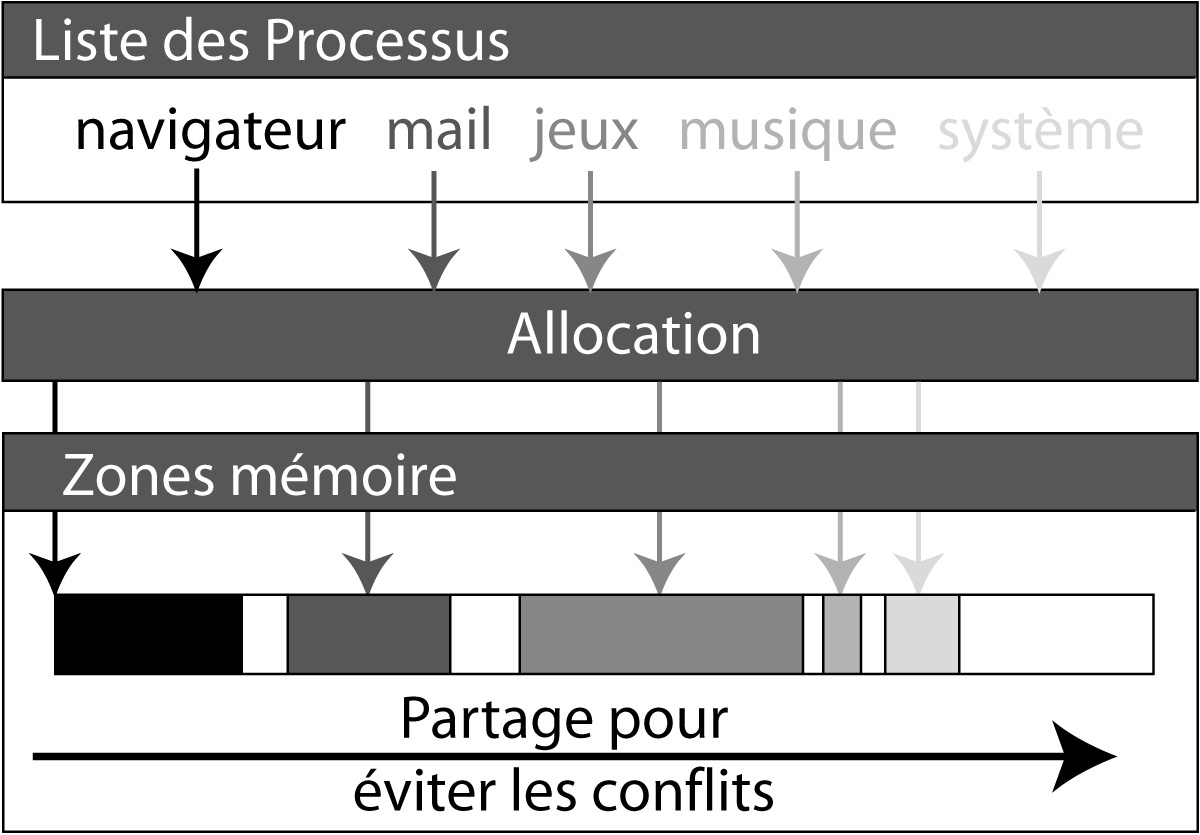
\includegraphics[width=5.5cm]{img/s03/Alloc_mem_2.jpg}
      \begin{block}{Allocation de zone mémoire}
        L'allocation permet:
        \begin{itemize}
        \item d'attribuer à chaque processus un espace de travail en
          mémoire,
        \item le système contraint le programme à écrire dans sa zone
          mémoire et ainsi,
        \item évite qu'un programme modifie les données d'un autre
          programme.
        \end{itemize}
      \end{block}
    \end{column}
  \end{columns}
\end{frame}
\begin{frame}{Gestion de la mémoire vive}
  \begin{center}
    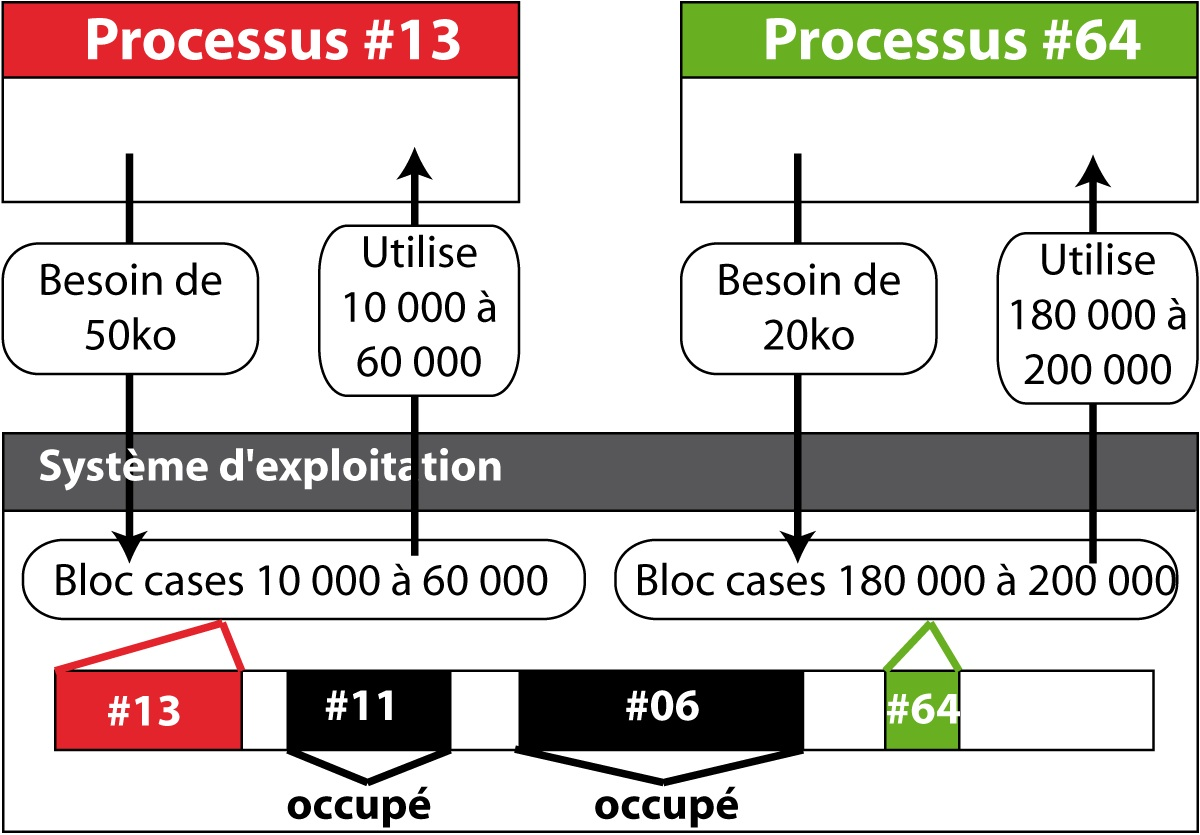
\includegraphics[width=7cm]{img/s03/Alloc_mem_3.jpg}
  \end{center}
  \begin{block}{Principes généraux de l'allocation}
    \begin{itemize}
    \item L'OS maintient une table des zones mémoires allouées à chaque
      processus. Ces zones sont réservées et ne peuvent être utilisées
      que par le processus parent.
    \item Lorsqu'il a besoin de mémoire, un processus demande à l'OS
      quelle zone il peut utiliser,
    \item L'OS lui attribue, en fonction de l'espace libre, un certain
      nombre de blocs mémoire.
    \item Les blocs mémoire attribués sont alors réservés.
    \end{itemize}
  \end{block}
\end{frame}
\subsection{Gestion de l'accès au CPU}
\begin{frame}{Gestion de l'accès au CPU}
  \begin{center}
    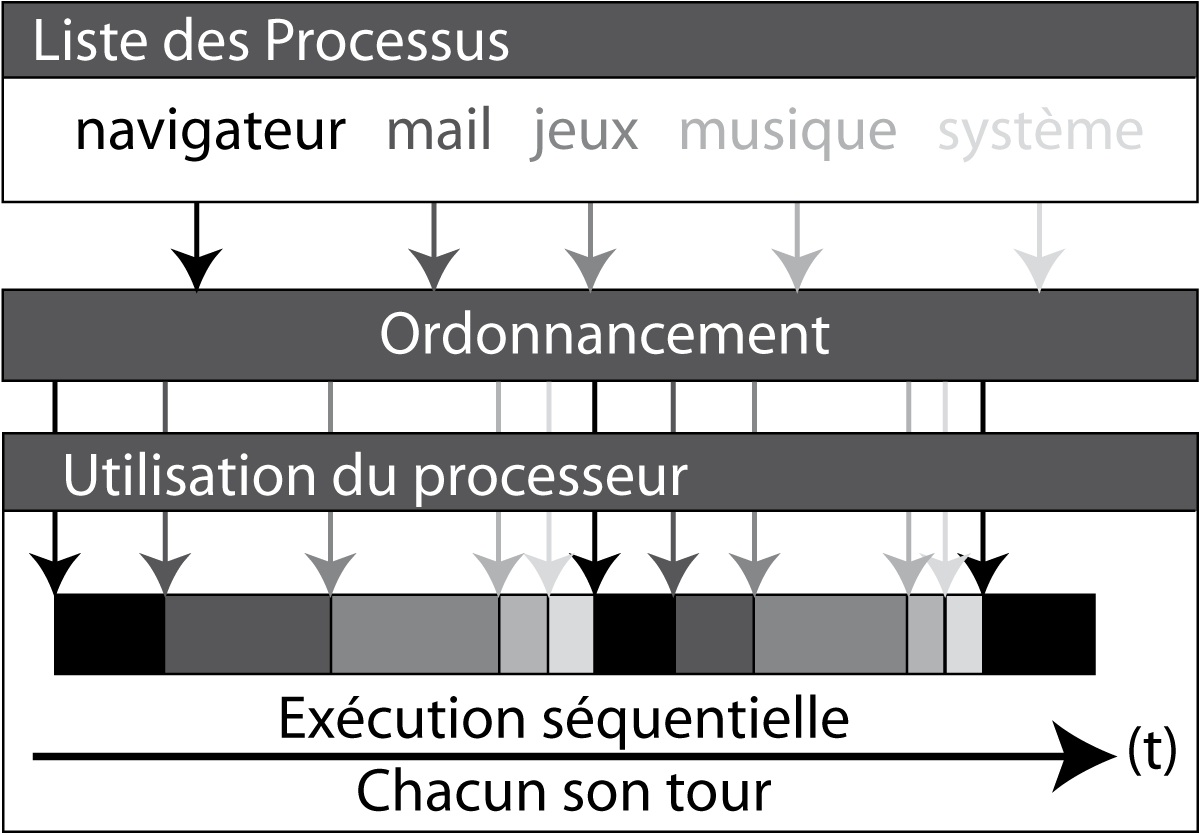
\includegraphics[width=7cm]{img/s03/Planificateur.jpg}
  \end{center}
  \begin{block}{Le planificateur gère le temps CPU attribué à chaque
      processus}
    \begin{itemize}
    \item Le CPU ne traite qu'un seul processus à la fois,
    \item Le planificateur permet l'alternance d'accès au CPU en
      attribuant une priorité à chaque processus.
    \item L'illusion d'exécution simultanée de plusieurs processus est
      donnée par une alternance rapide d'attribution de temps de calcul
      à chaque processus.
    \end{itemize}
  \end{block}
\end{frame}

\manpage{ps} \manpage{top}

\subsection{Processus en ligne de commande}
\begin{frame}{Processus en ligne de commande}
  \begin{block}{Occupation de la ligne de commande}
    \begin{itemize}
    \item Lorsque l'on tape une commande, la ligne de commande est
      bloquée (plus de prompt) jusqu'à la fin de l'exécution.
    \item La ligne de commande est à nouveau disponible ensuite.
    \end{itemize}
    \begin{center}
      \mprompt{ \prompt{sleep 20}{{\color{solarizedBlue}(\textit{il faut
              attendre 20 secondes avant l'apparition du nouveau
              prompt)\\\dots\\\dots}}} \prompt{\cursor}{} } \mprompt{
        \prompt{gedit}{{\color{solarizedBlue}(\textit{Il faut quitter
              l'application ou tuer le processus \lin{gedit} pour avoir
              un nouveau prompt)\\\dots\\\dots}}} }
    \end{center}
  \end{block}
\end{frame}

\begin{frame}{Libération de la ligne de commande}
  Deux façons possibles de lancer une instruction en tâche de fond:
  \begin{columns}
    \begin{column}{6cm}
      \begin{block}{Lancement en tâche de fond}
        \begin{itemize}
        \item Les commandes qui prennent beaucoup de temps peuvent être
          lancées en tâche de fond pour libérer la ligne de commande du
          shell.
        \item Pour lancer directement la commande en tâche de fond il
          suffit de faire suivre la commande du caractère
          {\color{red}\lin{\&}}. On retrouve immédiatement un nouveau
          prompt.
        \end{itemize}
        \vspace{20pt}
        \begin{center}
          \scriptsize{ \mpromptS{ \promptS{gedit \&}{}
              \promptS{\cursor}{} } }
        \end{center}
      \end{block}
    \end{column}
    \begin{column}{6cm}
      \begin{block}{Relégation en tâche de fond}
        \begin{itemize}
        \item Si une tâche déjà lancée occupe la ligne de commande, il
          est possible de suspendre son exécution en pressant la
          combinaison de touches \Ctrl\keystroke{Z}. La tâche est alors
          interrompue et on retrouve un nouveau prompt.
        \item Il est possible de relancer le processus en tâche de fond
          au moyen de la commande \lin{bg}.
        \end{itemize}
        \begin{center}
          \scriptsize{ \mpromptS{
              \promptS{gedit}{\^{}Z\\\string[1\string]\string$+ Stopped
                gedit} \promptS{bg}{\string[1\string]\string$+ gedit \&}
              \promptS{\cursor}{} } }
        \end{center}
      \end{block}
    \end{column}
  \end{columns}
\end{frame}

\begin{exercice}
  \begin{exercicelet}{Gestion des processus}
    Afin d'illustrer la gestion des processus nous allons utiliser la
    commande \texttt{sleep} pour simuler l'exécution de programmes dont
    l'exécution n'est pas immédiate. Pour se rappeler de son
    fonctionnement vous pouvez utiliser la commande man.
    \begin{enumerate}\setcounter{enumi}{\value{cnti}}
      \setcounter{cnti}{\value{enumi}}
    \item Évaluez l'instruction \verb|sleep 1000| puis tapez
      \Ctrl\keystroke{C}. Que se passe-t-il?
    \item Évaluez l'instruction \verb|sleep 1000 &| (n'oubliez pas le
      caractère \verb|&|). Que se passe-t-il?
    \item La commande ps permet d'afficher la liste de processus qui
      s'exécutent sur votre ordinateur. Un processus s'exécutant sous
      Linux est identifié par un numéro de processus, et par un
      propriétaire (celui qui a lancé le processus). Identifiez ces deux
      données lors de l'appel des commandes suivantes, donnez un
      explication à la différence des affichages (utilisez le man si
      nécessaire):
\begin{verbatim}
ps
ps -ef
\end{verbatim}
    \item Quel est le numéro de processus associé à la commande
      \verb|sleep 1000 &|?
    \end{enumerate}
  \end{exercicelet}
\end{exercice}
\begin{exercice}
  \begin{exercicelet}{Gestion des processus (suite)}
    \begin{enumerate}\setcounter{enumi}{\value{cnti}}
      \setcounter{cnti}{\value{enumi}}
    \item La commande kill permet de «~tuer~» (supprimer) un
      processus. Sa syntaxe d'utilisation est la suivante: \texttt{kill
        PID} où PID (Process ID) doit être remplacé par le numéro du
      processus à supprimer.  \setcounter{cnti}{\value{enumi}}
    \item Quelle commande permet de détruire le processus associé à
      la commande \verb|sleep 1000 &|?
    \item Tapez la commande \texttt{gedit} dans le terminal. Quel
      est l'effet sur la ligne de commande? Pouvez-vous saisir de
      nouvelle commandes?
    \item Après avoir lancé \texttt{gedit} (celui-ci étant en cours
      d'exécution), que se passe-t-il si on tape \Ctrl\keystroke{Z} dans
      le terminal qui a lancé \texttt{gedit}? Quel est l'effet sur le programme
      gedit (utilisez \texttt{ps} pour suivre l'état des processus)? Que se
      passe-t-il si vous tapez \texttt{bg}?
    \item Que fait la commande \texttt{top}?
    \item Exécutez la command \texttt{ps -ef f}. Examinez comment est
      construite la \emph{forêt} de processus. Repérez comment sont
      agencés les processus qui gèrent vos terminaux entre eux.
      \setcounter{cnti}{\value{enumi}}
    \end{enumerate}
  \end{exercicelet}
\end{exercice}
